\documentclass[11pt]{article}
\usepackage{cornell-notes}
\usepackage{mathtools}
\usepackage{needspace}
\usepackage{ragged2e}
\usepackage{adjustbox}
\usepackage{tikz}
\usetikzlibrary{arrows.meta,positioning}
\tcbuselibrary{most}
\geometry{letterpaper,margin=0.72in,headheight=15pt}
\setCornellCollection{Calculus Cornell Notes}
\setCornellUnitType{Chapter}
\setCornellUnitNumber{11}
\setCornellUnitTitle{Vectors and the Geometry of Space}

\definecolor{Ink}{HTML}{17324D}
\definecolor{Teal}{HTML}{147D78}
\definecolor{Sky}{HTML}{DDEEF1}
\definecolor{Cue}{HTML}{EEF2F5}
\definecolor{Warm}{HTML}{FFF3D6}
\definecolor{Alert}{HTML}{9D3C32}
\definecolor{Green}{HTML}{276749}
\definecolor{Rule}{HTML}{AAB8C2}
\hypersetup{colorlinks=true,linkcolor=Ink,urlcolor=Teal,pdfborder={0 0 0}}
\setlength{\parindent}{0pt}
\setlength{\parskip}{4pt}
\setlist{nosep,leftmargin=*}
\titleformat{\section}{\Large\bfseries\color{Ink}}{}{0pt}{}[\color{Teal}\titlerule]
\titleformat{\subsection}{\large\bfseries\color{Teal}}{}{0pt}{}
\pagestyle{fancy}
\fancyhf{}
\fancyhead[L]{\small\color{Ink}\textsc{Cornell Notes}}
\fancyhead[R]{\small\color{Teal}\nouppercase{\leftmark}}
\fancyfoot[L]{\footnotesize\color{Ink}Active recall $\bullet$ Worked reasoning $\bullet$ Verification}
\fancyfoot[R]{\footnotesize\color{Ink}\thepage\ of \pageref*{LastPage}}
\renewcommand{\headrulewidth}{0.5pt}
\renewcommand{\footrulewidth}{0.4pt}
\newcolumntype{Y}{>{\RaggedRight\arraybackslash}X}
\newtcolorbox{orientationbox}{enhanced,breakable,colback=Sky,colframe=Teal,boxrule=0.7pt,arc=2mm,title=Chapter orientation,fonttitle=\bfseries}
\newtcolorbox{sectionsummarybox}{enhanced,breakable,colback=white,colframe=Teal,boxrule=0.6pt,arc=1.5mm,left=2mm,right=2mm,top=1mm,bottom=1mm,title=Section synthesis,fonttitle=\bfseries\color{Teal}}
\newtcolorbox{warningbox}{enhanced,breakable,colback=Warm,colframe=Alert,boxrule=0.7pt,arc=1.5mm,title=Common error audit,fonttitle=\bfseries}
\newtcolorbox{checkbox}{enhanced,breakable,colback=white,colframe=Green,boxrule=0.7pt,arc=1.5mm,title=Verification habit,fonttitle=\bfseries}
\newcommand{\cornellcuehead}{\rowcolor{Ink}\color{white}\bfseries Cue / recall prompt & \color{white}\bfseries Notes / reasoning \\\endhead}
\newcommand{\cornellcuerow}[2]{\rowcolor{Cue}#1 & #2 \\\addlinespace[3pt]}
% Table-safe: delegates to the shared Cornell formula box (cornell-notes.sty),
% which cannot emit \pagebreak/\noalign inside longtable cells.
\newcommand{\formula}[1]{\CornellFormula[colback=Sky,colframe=Teal]{#1}}

\title{Chapter 11: Vectors and the Geometry of Space\\[2mm]\large Cornell Notes}
\author{}
\date{}
\hypersetup{pdftitle={Chapter 11: Vectors and the Geometry of Space - Cornell Notes},pdfauthor={},pdfsubject={Calculus study notes},pdfkeywords={calculus, Cornell notes, active recall}}
\begin{document}
\maketitle
\thispagestyle{fancy}
\begin{orientationbox}
Build three-dimensional geometry from vectors, products, lines, planes, surfaces, and alternative coordinate systems. These notes follow the complete local section sequence (751--818) and emphasize definitions, governing results, strategy selection, and verifiable reasoning.
\end{orientationbox}

\section{Prerequisite map}
\begin{minipage}[t]{0.42\textwidth}
\textbf{Bring forward}
\begin{itemize}
\item Coordinate geometry
\item Trigonometry
\item Systems of equations
\item Conic sections
\end{itemize}
\end{minipage}\hfill
\begin{minipage}[t]{0.54\textwidth}
\textbf{Chapter flow}
\begin{center}
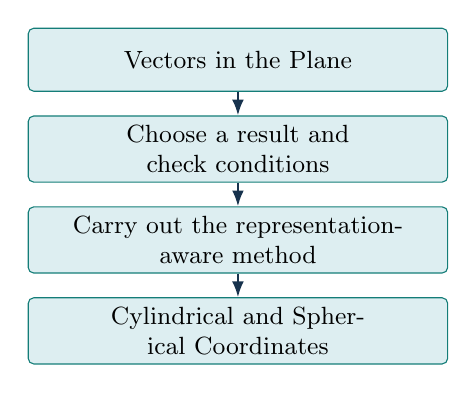
\begin{tikzpicture}[node distance=3mm, every node/.style={font=\small,align=center}, box/.style={draw=Teal,rounded corners=2pt,fill=Sky,minimum height=8mm,text width=0.42\textwidth}, arr/.style={-{Latex[length=2mm]},thick,draw=Ink}]
\node[box] (a) {Vectors in the Plane};
\node[box,below=of a] (b) {Choose a result and check conditions};
\node[box,below=of b] (c) {Carry out the representation-aware method};
\node[box,below=of c] (d) {Cylindrical and Spherical Coordinates};
\draw[arr] (a)--(b); \draw[arr] (b)--(c); \draw[arr] (c)--(d);
\end{tikzpicture}
\end{center}
\end{minipage}

\section{Learning objectives}
\begin{enumerate}
\item Explain the central objects and hypotheses in 11.1 and 11.7.
\item Translate among algebraic, graphical, numerical, and verbal representations.
\item Select an appropriate formula or theorem before beginning symbolic work.
\item Carry out multi-step calculations while preserving domain, sign, orientation, and units.
\item Diagnose common errors by testing assumptions and checking the result independently.
\item Synthesize the chapter's methods into a reusable problem-solving workflow.
\end{enumerate}

\section{11.1 Vectors in the Plane}
\begin{longtable}{C N}\cornellcuehead
\cornellcuerow{What is the governing idea in 11.1?}{A vector has magnitude and direction; components support geometric and algebraic operations.}
\cornellcuerow{Which result should be recalled?}{\formula{\|\mathbf v\|=\sqrt{v_1^2+v_2^2},\qquad \mathbf u=\mathbf v/\|\mathbf v\|}}
\cornellcuerow{How should a problem be organized?}{Translate points to displacement components, perform component operations, and separate vector results from scalar magnitudes.}
\cornellcuerow{What should be checked before accepting an answer?}{Confirm the hypotheses and domain, preserve units and orientation when relevant, and substitute or differentiate back into the defining relation.}
\end{longtable}
\begin{warningbox}Adding magnitudes instead of components ignores direction.\end{warningbox}
\begin{sectionsummarybox}A vector has magnitude and direction; components support geometric and algebraic operations. The operational habit is to translate points to displacement components, perform component operations, and separate vector results from scalar magnitudes.\end{sectionsummarybox}
\section{11.2 Space Coordinates and Vectors in Space}
\begin{longtable}{C N}\cornellcuehead
\cornellcuerow{What is the governing idea in 11.2?}{Three-dimensional coordinates extend distance, midpoint, sphere, and vector operations with a third component.}
\cornellcuerow{Which result should be recalled?}{\formula{\|\mathbf v\|=\sqrt{v_1^2+v_2^2+v_3^2}}}
\cornellcuerow{How should a problem be organized?}{Sketch coordinate traces when useful, compute component differences in a consistent order, and interpret spheres by center and radius.}
\cornellcuerow{What should be checked before accepting an answer?}{Confirm the hypotheses and domain, preserve units and orientation when relevant, and substitute or differentiate back into the defining relation.}
\end{longtable}
\begin{warningbox}A sign error in one component changes both direction and distance.\end{warningbox}
\begin{sectionsummarybox}Three-dimensional coordinates extend distance, midpoint, sphere, and vector operations with a third component. The operational habit is to sketch coordinate traces when useful, compute component differences in a consistent order, and interpret spheres by center and radius.\end{sectionsummarybox}
\section{11.3 The Dot Product of Two Vectors}
\begin{longtable}{C N}\cornellcuehead
\cornellcuerow{What is the governing idea in 11.3?}{The dot product connects components to angle, orthogonality, projection, and work.}
\cornellcuerow{Which result should be recalled?}{\formula{\mathbf u\cdot\mathbf v=\|\mathbf u\|\|\mathbf v\|\cos\theta}}
\cornellcuerow{How should a problem be organized?}{Compute the scalar product, use its sign to interpret angle, and divide by the squared magnitude for vector projection.}
\cornellcuerow{What should be checked before accepting an answer?}{Confirm the hypotheses and domain, preserve units and orientation when relevant, and substitute or differentiate back into the defining relation.}
\end{longtable}
\begin{warningbox}The dot product is scalar; confusing scalar and vector projections causes dimensional errors.\end{warningbox}
\begin{sectionsummarybox}The dot product connects components to angle, orthogonality, projection, and work. The operational habit is to compute the scalar product, use its sign to interpret angle, and divide by the squared magnitude for vector projection.\end{sectionsummarybox}
\section{11.4 The Cross Product of Two Vectors in Space}
\begin{longtable}{C N}\cornellcuehead
\cornellcuerow{What is the governing idea in 11.4?}{The cross product produces a perpendicular vector whose magnitude equals parallelogram area and whose orientation follows the right-hand rule.}
\cornellcuerow{Which result should be recalled?}{\formula{\|\mathbf u\times\mathbf v\|=\|\mathbf u\|\|\mathbf v\|\sin\theta}}
\cornellcuerow{How should a problem be organized?}{Set up the determinant carefully, check orthogonality by dot products, and halve the magnitude for triangle area.}
\cornellcuerow{What should be checked before accepting an answer?}{Confirm the hypotheses and domain, preserve units and orientation when relevant, and substitute or differentiate back into the defining relation.}
\end{longtable}
\begin{warningbox}Reversing operand order negates the vector, and the cross product is specific to three-dimensional vector calculus here.\end{warningbox}
\begin{sectionsummarybox}The cross product produces a perpendicular vector whose magnitude equals parallelogram area and whose orientation follows the right-hand rule. The operational habit is to set up the determinant carefully, check orthogonality by dot products, and halve the magnitude for triangle area.\end{sectionsummarybox}
\section{11.5 Lines and Planes in Space}
\begin{longtable}{C N}\cornellcuehead
\cornellcuerow{What is the governing idea in 11.5?}{A line uses a point and direction; a plane uses a point and normal vector.}
\cornellcuerow{Which result should be recalled?}{\formula{\mathbf r=\mathbf r_0+t\mathbf v,\qquad \mathbf n\cdot(\mathbf r-\mathbf r_0)=0}}
\cornellcuerow{How should a problem be organized?}{Extract direction or normal data, write vector and component forms, and solve parameters to test intersection or distance.}
\cornellcuerow{What should be checked before accepting an answer?}{Confirm the hypotheses and domain, preserve units and orientation when relevant, and substitute or differentiate back into the defining relation.}
\end{longtable}
\begin{warningbox}A plane's normal is not a direction lying in the plane.\end{warningbox}
\begin{sectionsummarybox}A line uses a point and direction; a plane uses a point and normal vector. The operational habit is to extract direction or normal data, write vector and component forms, and solve parameters to test intersection or distance.\end{sectionsummarybox}
\section{11.6 Surfaces in Space}
\begin{longtable}{C N}\cornellcuehead
\cornellcuerow{What is the governing idea in 11.6?}{Equations in three variables describe cylinders and quadric surfaces whose traces reveal geometry.}
\cornellcuerow{Which result should be recalled?}{\formula{Ax^2+By^2+Cz^2+Dz+\cdots=K}}
\cornellcuerow{How should a problem be organized?}{Complete squares, inspect missing variables, sketch coordinate-plane traces, and classify signs and degeneracies.}
\cornellcuerow{What should be checked before accepting an answer?}{Confirm the hypotheses and domain, preserve units and orientation when relevant, and substitute or differentiate back into the defining relation.}
\end{longtable}
\begin{warningbox}A missing variable usually signals a cylinder, not a bounded surface.\end{warningbox}
\begin{sectionsummarybox}Equations in three variables describe cylinders and quadric surfaces whose traces reveal geometry. The operational habit is to complete squares, inspect missing variables, sketch coordinate-plane traces, and classify signs and degeneracies.\end{sectionsummarybox}
\section{11.7 Cylindrical and Spherical Coordinates}
\begin{longtable}{C N}\cornellcuehead
\cornellcuerow{What is the governing idea in 11.7?}{Alternative coordinates exploit axial or radial symmetry and map to rectangular coordinates through trigonometry.}
\cornellcuerow{Which result should be recalled?}{\formula{x=\rho\sin\phi\cos\theta,\ y=\rho\sin\phi\sin\theta,\ z=\rho\cos\phi}}
\cornellcuerow{How should a problem be organized?}{Choose the system matching symmetry, convert representative boundaries, and state angle ranges to remove ambiguity.}
\cornellcuerow{What should be checked before accepting an answer?}{Confirm the hypotheses and domain, preserve units and orientation when relevant, and substitute or differentiate back into the defining relation.}
\end{longtable}
\begin{warningbox}Conventions for the spherical angle $\phi$ vary; the coordinate definitions must be fixed before use.\end{warningbox}
\begin{sectionsummarybox}Alternative coordinates exploit axial or radial symmetry and map to rectangular coordinates through trigonometry. The operational habit is to choose the system matching symmetry, convert representative boundaries, and state angle ranges to remove ambiguity.\end{sectionsummarybox}

\section{Definitions and theorem register}
\small
\begin{longtable}{@{}>{\RaggedRight\arraybackslash}p{0.24\textwidth}>{\RaggedRight\arraybackslash}p{0.40\textwidth}>{\RaggedRight\arraybackslash}p{0.29\textwidth}@{}}
\toprule
\textbf{Topic} & \textbf{Meaning and conditions} & \textbf{Canonical form}\\
\midrule\endhead
11.1 Vectors in the Plane & A vector has magnitude and direction; components support geometric and algebraic operations. & \adjustbox{max width=\linewidth}{\(\displaystyle \|\mathbf v\|=\sqrt{v_1^2+v_2^2},\qquad \mathbf u=\mathbf v/\|\mathbf v\|\)} \\\addlinespace[2pt]
11.2 Space Coordinates and Vectors in Space & Three-dimensional coordinates extend distance, midpoint, sphere, and vector operations with a third component. & \adjustbox{max width=\linewidth}{\(\displaystyle \|\mathbf v\|=\sqrt{v_1^2+v_2^2+v_3^2}\)} \\\addlinespace[2pt]
11.3 The Dot Product of Two Vectors & The dot product connects components to angle, orthogonality, projection, and work. & \adjustbox{max width=\linewidth}{\(\displaystyle \mathbf u\cdot\mathbf v=\|\mathbf u\|\|\mathbf v\|\cos\theta\)} \\\addlinespace[2pt]
11.4 The Cross Product of Two Vectors in Space & The cross product produces a perpendicular vector whose magnitude equals parallelogram area and whose orientation follows the right-hand rule. & \adjustbox{max width=\linewidth}{\(\displaystyle \|\mathbf u\times\mathbf v\|=\|\mathbf u\|\|\mathbf v\|\sin\theta\)} \\\addlinespace[2pt]
11.5 Lines and Planes in Space & A line uses a point and direction; a plane uses a point and normal vector. & \adjustbox{max width=\linewidth}{\(\displaystyle \mathbf r=\mathbf r_0+t\mathbf v,\qquad \mathbf n\cdot(\mathbf r-\mathbf r_0)=0\)} \\\addlinespace[2pt]
11.6 Surfaces in Space & Equations in three variables describe cylinders and quadric surfaces whose traces reveal geometry. & \adjustbox{max width=\linewidth}{\(\displaystyle Ax^2+By^2+Cz^2+Dz+\cdots=K\)} \\\addlinespace[2pt]
11.7 Cylindrical and Spherical Coordinates & Alternative coordinates exploit axial or radial symmetry and map to rectangular coordinates through trigonometry. & \adjustbox{max width=\linewidth}{\(\displaystyle x=\rho\sin\phi\cos\theta,\ y=\rho\sin\phi\sin\theta,\ z=\rho\cos\phi\)} \\\addlinespace[2pt]
\bottomrule
\end{longtable}
\normalsize

\section{Formula and method sheet}
\small
\begin{longtable}{@{}>{\RaggedRight\arraybackslash}p{0.08\textwidth}>{\RaggedRight\arraybackslash}p{0.48\textwidth}>{\RaggedRight\arraybackslash}p{0.37\textwidth}@{}}
\toprule
\textbf{Sec.} & \textbf{Method sequence} & \textbf{Stop-and-check trigger}\\
\midrule\endhead
11.1 & Translate points to displacement components, perform component operations, and separate vector results from scalar magnitudes. & Adding magnitudes instead of components ignores direction. \\\addlinespace[2pt]
11.2 & Sketch coordinate traces when useful, compute component differences in a consistent order, and interpret spheres by center and radius. & A sign error in one component changes both direction and distance. \\\addlinespace[2pt]
11.3 & Compute the scalar product, use its sign to interpret angle, and divide by the squared magnitude for vector projection. & The dot product is scalar; confusing scalar and vector projections causes dimensional errors. \\\addlinespace[2pt]
11.4 & Set up the determinant carefully, check orthogonality by dot products, and halve the magnitude for triangle area. & Reversing operand order negates the vector, and the cross product is specific to three-dimensional vector calculus here. \\\addlinespace[2pt]
11.5 & Extract direction or normal data, write vector and component forms, and solve parameters to test intersection or distance. & A plane's normal is not a direction lying in the plane. \\\addlinespace[2pt]
11.6 & Complete squares, inspect missing variables, sketch coordinate-plane traces, and classify signs and degeneracies. & A missing variable usually signals a cylinder, not a bounded surface. \\\addlinespace[2pt]
11.7 & Choose the system matching symmetry, convert representative boundaries, and state angle ranges to remove ambiguity. & Conventions for the spherical angle $\phi$ vary; the coordinate definitions must be fixed before use. \\\addlinespace[2pt]
\bottomrule
\end{longtable}
\normalsize

\section{Common errors and diagnostic checks}
\begin{warningbox}
\begin{itemize}
\item \textbf{11.1:} Adding magnitudes instead of components ignores direction.
\item \textbf{11.2:} A sign error in one component changes both direction and distance.
\item \textbf{11.3:} The dot product is scalar; confusing scalar and vector projections causes dimensional errors.
\item \textbf{11.4:} Reversing operand order negates the vector, and the cross product is specific to three-dimensional vector calculus here.
\item \textbf{11.5:} A plane's normal is not a direction lying in the plane.
\item \textbf{11.6:} A missing variable usually signals a cylinder, not a bounded surface.
\item \textbf{11.7:} Conventions for the spherical angle $\phi$ vary; the coordinate definitions must be fixed before use.
\end{itemize}
\end{warningbox}
\begin{checkbox}
Before accepting any result: state the relevant domain; check theorem hypotheses; estimate sign and scale; preserve units and orientation; and verify by substitution, differentiation, a limiting case, or a second representation.
\end{checkbox}

\section{Chapter synthesis}
Build three-dimensional geometry from vectors, products, lines, planes, surfaces, and alternative coordinate systems. The chapter begins with \textbf{Vectors in the Plane} and culminates in \textbf{Cylindrical and Spherical Coordinates}. Across the sequence, the most reliable workflow is to identify the mathematical object, choose a representation, state the governing result with its hypotheses, compute without dropping restrictions, and audit the answer against the original definition. Vector geometry becomes dependable when every scalar, direction, normal, coordinate convention, and geometric equation is interpreted before it is manipulated.

\section{Self-test questions}
\begin{enumerate}
\item Explain the central distinction or object in 11.1, using both words and notation.
\item State the main formula or result from 11.2 and identify every hypothesis or restriction needed for its use.
\item Describe the problem-solving procedure for 11.3. What is the strongest independent check?
\item Compare the roles of Vectors in the Plane and Cylindrical and Spherical Coordinates within this chapter.
\item Reconstruct the governing formula for 11.4 from its geometric or analytic meaning.
\item Choose one method in the chapter and explain how its output should be interpreted, including units or orientation when applicable.
\item Scenario: A student working on 11.1 produces a polished calculation but makes this error: Adding magnitudes instead of components ignores direction. Diagnose the earliest invalid step and repair the workflow.
\item Scenario: A solution in 11.2 quotes the displayed formula without checking conditions. Which conditions must be checked, and what could fail if they are absent?
\item Construct a concept map linking a representation, a governing result, a computation, and a verification check from this chapter.
\item Design a two-part test for mastery: one conceptual prompt and one calculation. State what evidence would count as a complete answer.
\end{enumerate}

\Needspace{8\baselineskip}
\section{Answer key}
\small
\begin{enumerate}
\item A complete response identifies A vector has magnitude and direction; components support geometric and algebraic operations. It should connect that meaning to \(\|\mathbf v\|=\sqrt{v_1^2+v_2^2},\qquad \mathbf u=\mathbf v/\|\mathbf v\|\) and state the relevant domain.
\item The organizing result is \(\|\mathbf v\|=\sqrt{v_1^2+v_2^2+v_3^2}\). The solver must check that the quantities are defined and that the assumptions named in 11.2 hold before applying it.
\item Use this sequence: Compute the scalar product, use its sign to interpret angle, and divide by the squared magnitude for vector projection. The strongest check is to return to the defining relation or differentiate/substitute the result, as appropriate.
\item Vectors in the Plane establishes a vector has magnitude and direction; components support geometric and algebraic operations. Cylindrical and Spherical Coordinates extends the chapter to alternative coordinates exploit axial or radial symmetry and map to rectangular coordinates through trigonometry. The connection is the reuse of the same representations under a broader method.
\item The formula \(\|\mathbf u\times\mathbf v\|=\|\mathbf u\|\|\mathbf v\|\sin\theta\) follows by translating the defining geometric or rate relationship into symbols; each factor records a distinct change or scale.
\item Interpretation must name what varies, with respect to what, and on which domain. A numerical value without units, sign, direction, or interval information is incomplete whenever those features are part of the modeled quantity.
\item The earliest fault is the unverified assumption described by this warning: Adding magnitudes instead of components ignores direction. Restart by following this procedure: Translate points to displacement components, perform component operations, and separate vector results from scalar magnitudes.
\item The formula \(\|\mathbf v\|=\sqrt{v_1^2+v_2^2+v_3^2}\) is conditional, not decorative. Check domain, differentiability or integrability as relevant, boundary or orientation requirements, and nonzero denominators before drawing a conclusion.
\item One valid map is: the representation in 11.1 identifies the object; the result in 11.2 supplies a rule; the method in 11.3 carries out the computation; the check in 11.7 tests the conclusion against its definition.
\item The conceptual prompt should require explanation of a definition and its hypotheses. The calculation should require method selection rather than direct substitution. Full evidence includes setup, justified transformations, a result, and an independent check.
\end{enumerate}
\normalsize

\section{Key-term recap}
\small
\begin{longtable}{@{}>{\RaggedRight\arraybackslash}p{0.29\textwidth}>{\RaggedRight\arraybackslash}p{0.64\textwidth}@{}}
\toprule
\textbf{Term} & \textbf{Working meaning}\\
\midrule\endhead
Vectors in the Plane & A vector has magnitude and direction; components support geometric and algebraic operations. \\\addlinespace[2pt]
Space Coordinates and Vectors in Space & Three-dimensional coordinates extend distance, midpoint, sphere, and vector operations with a third component. \\\addlinespace[2pt]
The Dot Product of Two Vectors & The dot product connects components to angle, orthogonality, projection, and work. \\\addlinespace[2pt]
The Cross Product of Two Vectors in Space & The cross product produces a perpendicular vector whose magnitude equals parallelogram area and whose orientation follows the right-hand rule. \\\addlinespace[2pt]
Lines and Planes in Space & A line uses a point and direction; a plane uses a point and normal vector. \\\addlinespace[2pt]
Surfaces in Space & Equations in three variables describe cylinders and quadric surfaces whose traces reveal geometry. \\\addlinespace[2pt]
Cylindrical and Spherical Coordinates & Alternative coordinates exploit axial or radial symmetry and map to rectangular coordinates through trigonometry. \\\addlinespace[2pt]
\bottomrule
\end{longtable}
\normalsize

\enlargethispage{4\baselineskip}
\begin{tcolorbox}[title=One-sentence takeaway,fonttitle=\bfseries,colback=Ink,colframe=Ink,coltext=white,coltitle=white,arc=2mm,boxrule=0pt]
\centering\bfseries Vector geometry becomes dependable when every scalar, direction, normal, coordinate convention, and geometric equation is interpreted before it is manipulated.
\end{tcolorbox}
\end{document}
